


\chapter{%State-space Covariates
%Modeling Spatial Variation in Density Using State-Space Covariates
Modeling Spatial Variation in Density
}
\markboth{Spatial Variation in Density}{}
\label{chapt.state-space}

\vspace{0.3cm}

Underlying all spatial capture-recapture models is a point process
model that describes the distribution of individual activity
centers (${\bf s}$) within the state-space ($\cal{S}$).
%, which is
%typically a two-dimensional polygon defining the study area.
Point process models are charcterized by $\mathcal{S}$ and by an
intensity parameter defined at each location in $\mathcal{S}$. In the
case of SCR models, the intensity parameter is population density. If this
intensity is constant, density is constant throughout $\mathcal{S}$
and the point process is said to be homogeneous.
Thus far we have focused our
attention on the homogeneous binomial point process whose realized
values are:
${\bf s}_i \sim \mbox{Unif}({\cal S}), i=1,2,\dots,N$, where $N$ is the
size of the population. This is a model of
``spatial-randomness''\footnote{The phrase ``complete
  spatial-randomness'' is reserved for the homogeneous Poisson point
  process}
because the point process intensity is constant %across the study area
and the activity centers do not interact with one another.

The spatial-randomness assumption is often viewed as restrictive
because ecological processes such as
territoriality and habitat selection can result in non-uniform
distributions of organisms. We have argued, however, that this
assumption is less restrictive than may be recognized because the
homogeneous point process actually allows for infinite
possible configurations of activity centers. Furthermore, given enough data,
the uniform prior will have very little influence on the estimated
locations of activity centers. Nonetheless, the homogeneous point
process model does not allow one to model population density using
covariates, which is a central objective of much ecological research.
For example, a homogeneous point process model
may result in a density surface map indicating that individuals were
more abundant in one habitat than another, but it does not do so
explicitly and so cannot be used to make predictions about
habitat-specific abundance in other regions. A more direct approach would be to replace
the homogeneous model with an inhomogeneous model in which the point process
intensity varies spatially.

In this chapter, we cover methods % we present a method
for fitting inhomogeneous Poisson and binomial
point process models by modeling
the intensity parameter as a function of
covariates in much the same way as is done with generalized linear
models. The covariates we consider differ
from those covered in previous chapters, which were typically
attributes of the animal ({\it e.g.} sex or age) or the trap ({\it
  e.g.} baited or not) and were used to model movement or encounter
rate. In contrast, here we wish to
model covariates that are defined for all points in
$\cal{S}$, which we will refer to as
state-space covariates or density covariates. These may
include continuous covariates such as elevation, or discrete
covariates such as habitat type.

Inhomogeneous Poisson point process models were discussed in the original
formulation of SCR models \citep{efford:2004} and were described in
detail by \citet{borchers_efford:2008}. Our approach is
similar to that of \citet{borchers_efford:2008}, except that we use a binomial
rather than a Poisson model for $N$ because the binomial model is
easily integrated into our MCMC algorithm.  %data augmentation scheme
%and is consistent
%with the objective of determining how a {\it fixed} number of activity
%centers are distributed with respect to covariates.
The method we use to fit inhomogeneous point process
models %within our MCMC algorithm
is simple---we
replace the uniform prior with a prior describing the
distribution of the $N$ activity centers conditional on the
covariates. Development of this prior, which does not have a
standard form, is a central component of this chapter. First we
begin with a review of homogeneous point process models.


\section{Homogeneous point process revisited}

The homogeneous Poisson point process is \textit{the} model of ``complete
spatial randomness'' and is often used in ecology as a null model
to test for departures from randomness
\citep{cressie:1992, diggle:2003, illian_etal:2008}.
%Given its central role in spatial ecology, it is helpful to describe it briefly and
%compare it with the binomial model that we use in when conducting
%Bayesian analysis of SCR models.
As with all homogeneous point process models, the Poisson model
asserts that the realized points do not interact with each other in
any way, e.g. they neither attract nor repel one another.
What is unique about this model, however, is that the number of realized points in $\mathcal{S}$ is
Poisson distributed: $N \sim \text{Poisson}(\mu|\mathcal{S}|)$ where $\mu>0$ is
the intensity parameter and $|\mathcal{S}|$ is the area of the
state-space. The intensity parameter $\mu$ is defined as the expected number
of points in some infinitesimally small area. In other words, it is
the density of points, and thus multiplying the intensity by the area
of some region yields the expected number of points in that region. In
SCR settings, $N$ is population size in the state-space and $\mu$ is
population density.
%Another important characteristic
%of the homogenous Poisson point
%process is that the points neither repel or attract
%each other. %, and that the number of points
%in two disjunct regions of $\mathcal{S}$ are independent of one another.
%describes the expected number
%of points per unit area. The number . Specifically,
%$\mathbb{E}[n(B)] = A(B)\mu$ where $A(B)$ is the area of region $B$.
%This just says that
%the expected number of points is the area of $B$
%multiplied by the intensity parameter.
%This is one
%of the distinctions between the Poisson model and the binomial model,
%for which the counts $\{n(B_k)\}$ are not i.i.d., as we will explain
%shortly.

Unlike the Poisson point process, the
binomial point process assumes that $N$ is fixed, not random,
%In other words, the binomial point process conditions on $N$,
as is illustrated by this simple \R~code that generates realizations
from Poisson and binomial point processes in the unit square
($\mathcal{S} = [0,1]\times[0,1]$):
\begin{verbatim}
Area <- 1                          # Area of unit square
muP <- 4                           # intensity
nP <- rpois(1, muP*Area)           # number of points: random
PPP <- cbind(runif(nP), runif(nP)) # Poisson point process

nB <- 4                            # number of points: fixed
muB <- nB/Area                     # intensity
BPP <- cbind(runif(nB), runif(nB)) # binomial point process
\end{verbatim}
Both of these models are homogeneous because the intensity parameter
is constant ($\mu=4$ in both cases) and the $N$ points do not interact
with each other in any way. The key distinction is that $N$ is random
in the former and fixed in the latter.

Another difference between the Poisson and binomial models is that if the
state-space is divided into $K$ disjunct regions, the number of points in each
region $n(B_k): k=1,\dots,K$; are independent and identically
distributed (i.i.d.) under the Poisson model but not under the
binomial model. To see this, first note that in the Poisson case,
the counts are simply distributed as $n(B_k) \sim
\text{Poisson}(\mu|B_k|)$, where $|B_k|$ is the area of the region
$B_k|$. For the homogeneous binomial point process, $n(B_k) \sim
\text{Binomial}(N, \pi(B_k))$ where $\pi(B_k)$ is the proportion of
the state-space in the region $B_k$; however, these counts are not
i.i.d. because the number of points in one region is informative
about the number of points in another region. For example, if we know
that $N=10$ and that there are 7 points outside the region $B_1$,
then we can say with certainty that $B_1 = 10 - 7 = 3$.

Fig.~\ref{state-space.fig.homo} is meant to further illustrate the characteristics
of the binomial model. The left panel shows a realization from a
homogeneous binomial point process with $N=50$. The right panel shows
the same realization, except that the state-space has been discretized
into 25 equally-sized disjunct regions, and the counts in each region
are shown. Since the regions are the same
size, $\pi(B_k) = 1/25$, and the expected number of point in each
region is 2: $\mathbb{E}(n(B_k)) = N\pi(B_k) = 50/25$, which
happens to be the empirical mean in this instance. However, as
previously stated, these counts are not
independent realizations from a binomial distribution since $\sum_k
n(B_k) = N$. Instead, the model for the entire vector is multinomial:
$\{n(B_1), n(B_2), \dots, n(B_k)\} \sim \mbox{Multinom}(N, \{p(B_1), p(B_2), \dots,
p(B_K) \})$ \citep{illian_etal:2008}. If you need a refresher on the
multinomial distribution, refer to Sec.~\ref{modeling.sec.multinom}, and
consider the following \R~code, which generates counts such as those
seen in Fig.~\ref{state-space.fig.homo}:
\begin{verbatim}
n.Bk <- rmultinom(1, size=50, prob=rep(1/25, 25))
matrix(n.Bk, 5, 5)
\end{verbatim}
The dependence among counts has virtually
no practical consequence when the number of pixels is large. For
example, if there are 100 pixels, the number of points in one pixels
carries very little information about the expected number of points in another
pixel. However, if there are only 2 pixels, then clearly the number of
points in one pixel allows one to determine how many points will occur in the
remaining pixel.

\begin{figure}%[ht!]
\centering
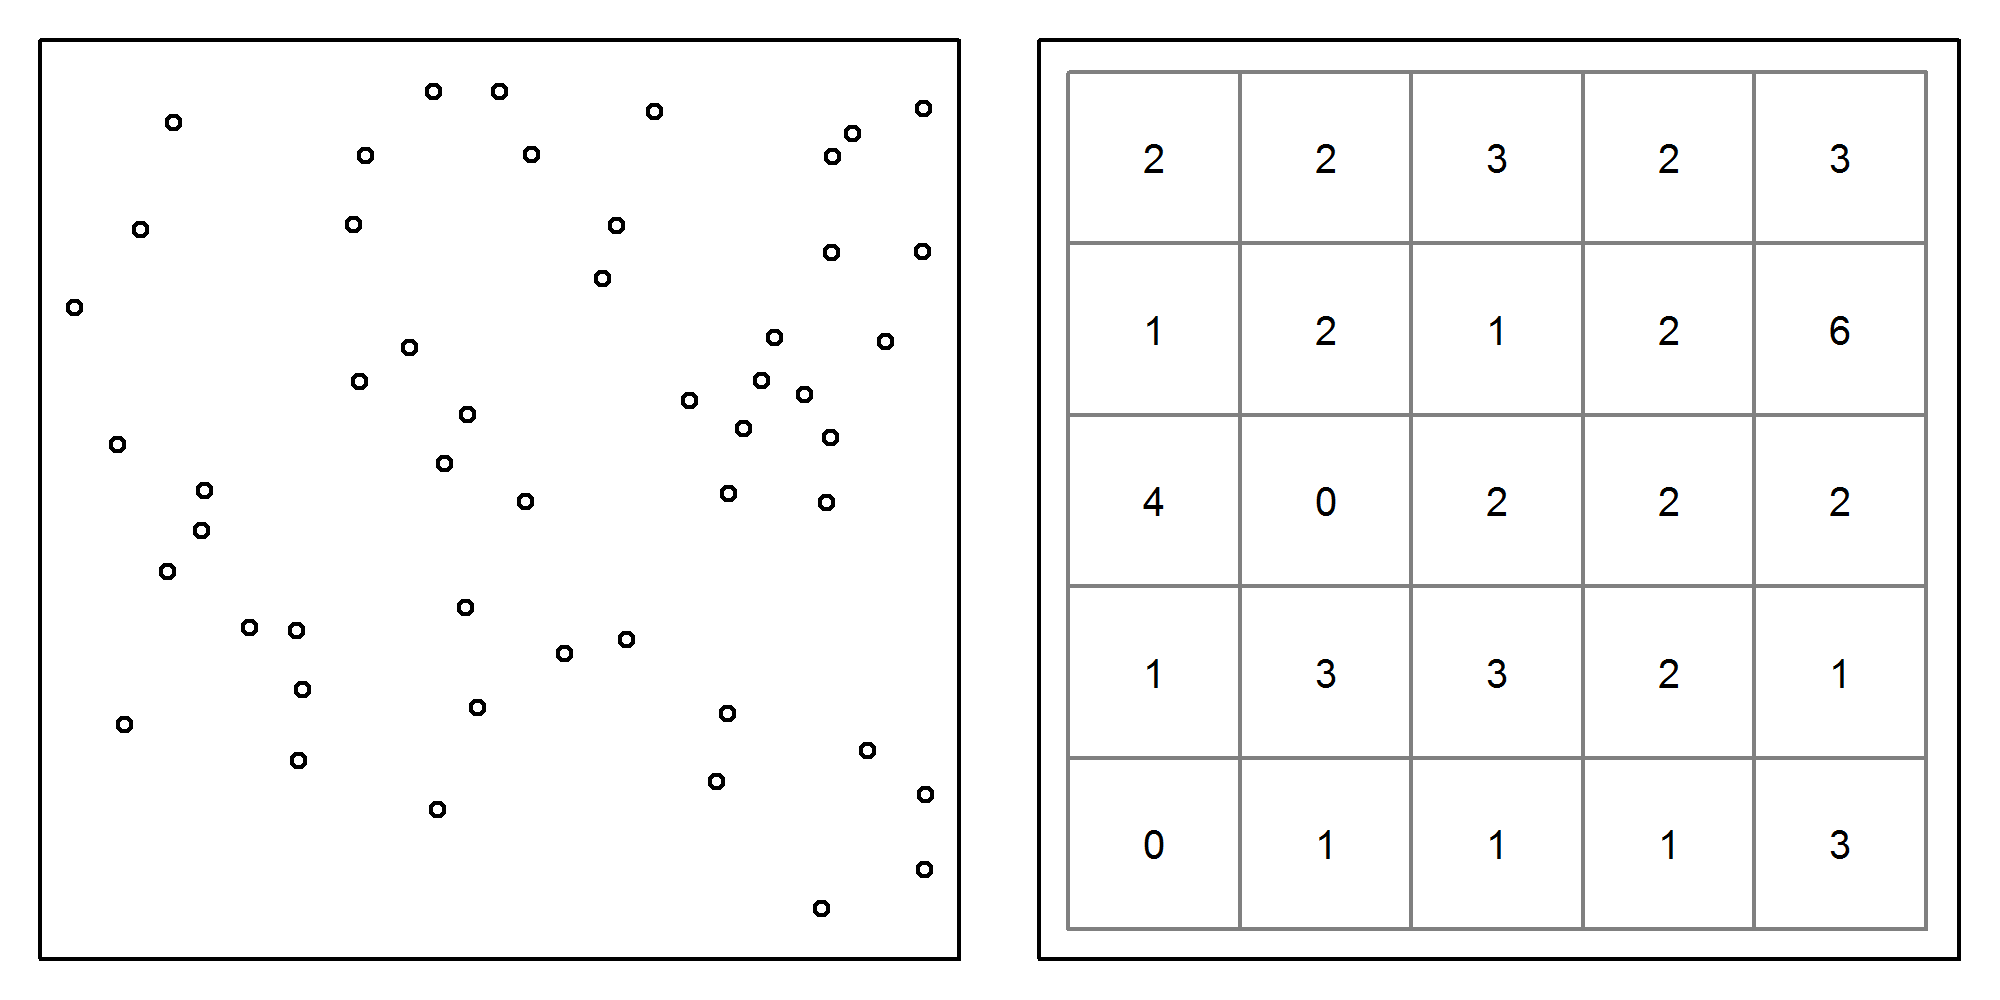
\includegraphics[width=5in,height=2.5in]{Ch11/figs/homoPlots}
\label{state-space.fig.homo}
\caption{Homogeneous binomial point process with $N$=50 points
  represented in continuous and discrete space.}
\end{figure}

\begin{comment}
  The discrete space representation of %the binomial
  point processes is of practical importance when fitting SCR models
  because spatial covariates are almost always represented in a
  discrete-space format called ``rasters'' in GIS-speak. In such
  cases, we need to change the the definition of the prior for
  activity centers from the probability that $\bf s$ occurs at some
  point in space to the probability that $\bf s$ occurs in some pixel
  of the raster. To do this, we can change the prior from the uniform
  distribution to the multinomial distribution, or equivalently, the
  categorical distribution as demonstrated in
  Sec.~\ref{modeling.sec.discrete}.
  % In the latter case, the activity center is simply defined as an
  % integer representing pixel ``id''.
\end{comment}

So far in this chapter we have sketched out the the homogeneous
Poisson and binomial point process models in general terms. Now we
need to expound upon their relevance to SCR models before we move on
to the inhomogeneous models.
In SCR a model with a homogeneous point process, the intensity
parameter $\mu$ is population density, and $N$ is
population size\footnote{Defined as the number of activity centers in
$\mathcal{S}$}. This is true regardless of whether we consider the
Poisson or the binomial models, and since $N$ is always unknown, one
might wonder why we are discussing the binomial model at all. Indeed,
the binomial model was not mentioned by \citet{efford:2004} or
\citet{borchers_efford:2008}. Instead, they focused exclusively on the
Poisson model and estimation of $\mu$, with $N$ being regarded as a
derived parameter.

In our work, we typically adopt the binomial model simply
because it is easy to implement using MCMC based on data
augmentation. And while $N$ is truly unkown, we use an upper bound $M$
which is fixed. Thus, the standard point process we use can be thought
of in two ways. First, it is a binomial point process with $M$
points. Second, in terms of $N$, it is a thinned binomial point
process, where $\psi$ is the thinning parameter. With this in mind,
the only real difference between the Poisson and binomial models, as
implemented in SCR contexts, is that in the former, we have
$N \sim \text{Poisson}(\mu|\mathcal{S})$, and it the latter we have
$N \sim \text{Binomial}(M, \psi)$. In other words, we just have a
different prior on $N$, and when using MCMC, the binomial prior is
much more convienient becuase it fixes the size of the parameter space
and makes it easy to include individual-specific covariates, among
other model extensions.
It is also worth remembering that the Poisson
distribution is the limit of the binomial distribution when, in this
case, $M$ is very high and $\psi$ is very low. In this case, there is
virtually no difference between the Poisson and binomial models.

Hopefully you noticed that the intensity parameter $\mu$ does not
appear in the binomial model for $N$ shown above. Instead, we see the
data augmentation parameter $\psi$, which has been used throughout
this book. What then is the relationship between $\psi$ and $\mu$?
As first discussed in Chapt.\ref{chapt.scr0}, under data augmentation,
the expected value of $N$ is $\mathbb{E}[N] = M\psi$. But, from this
chapter, we also know that the
expected value of $N$ can be written in terms of $\mu$ as
$\mathbb{E}[N] = \mu|\mathcal{S}|$. Therefore,
$\psi = \mu|\mathcal{S}| / M$ and hence we can directly estimate $\mu$
rather than $\psi$ if we so desire -- and we will so desire in the next
section where the objective is to model $\mu$ as a function of
spatially-referenced covariates. The following \R~code demontrates
these concepts:
\begin{verbatim}
Area <- 1                  # Area of state-space
M <- 100                   # Data augmentation size
mu <- 10                   # Intensity (points per area)
psi <- (mu*Area)/M         # Data augmentation parameter (thinning rate)
N <- rbinom(M, 1, psi)     # Realized value of N under binomial prior
cbind(runif(N), runif(N))  # Coordinates of activity centers
\end{verbatim}

We conclude this section by pointing
out Table\ref{state-space.tab.pvb}, which highlights the differences
of the homogeneous Poisson and binomial point process models as they
relate to SCR. % XXXX Need to fill in this table XXXX

\begin{table}
  \centering
  \caption{Characteristics of the homogeneous Poisson and binomial point processes. }
  \begin{tabular}{lccc}
    \hline
    & $\mathbb{E}[N]$  & $\mu$  &  \\
    \hline
    Poisson  &    &  &  \\
    Binomial &    &  &  \\
    \hline
  \end{tabular}
  \label{state-space.tab.pvb}
\end{table}

\section{Inhomogeneous binomial point process}

The principal difference between homogeneous and inhomogeneous point
processes is that the intensity parameter $\mu$ is allowed to vary spatially
in the inhomogeneous model. Thus, rather than $\mu$ being a fixed constant,
it is now a function defined at each point $x \in
\mathcal{S}$. Typically, the function is determined by
spatially-referenced covariates and a vector of regression
coefficients $\bm \beta$, thus we denote the function $\mu(x,
\bm{\beta})$. Since the intensity must be %strictly
positive, and because the natural logarithm is the canonical link
function of the Poisson generalized linear model, it is natural to
consider the following model:
\begin{equation}
  \log(\mu(x, \beta)) = \beta_0 + \sum_{v=1}^V \beta_v z(x)_v, \quad  s \in \cal{S}
  \label{state-space.eq.loglin}
\end{equation}
which says that we have $V$ covariates and $\beta_v$ is the regression coefficient for covariate
$z(s)_v$. To be clear, $z(s)_v$ is the value of a covariate, such as
habitat type or elevation, at location $s$, and it assumed to be
defined at all locations in the state-space.
This equation should look
familiar because it is the standard linear predictor used in log-linear
GLMs.

For a homogeneous Poisson point process, the expected number of points
in the state-space is $\mathbb{E}[N] = \mu|\mathcal{S}|$ for a
homogeneous point process.  , , but what is
it in the inhomogeneous case in which $\mu$ is no longer constant?
Contemplating a discrete state-space is useful for figuring this out.


\begin{comment}
  In the context of spatial capture-recapture models, if one assumes
  an inhomogeneous Poisson point process for the activity centers,
  then each of the $\bm \beta$ parameters is identifiable, and the
  intercept $\beta_0$ is interpretted as population density when all
  covariates equal zero. However, in the case of an inhomogeneous
  binomial point process, in which we condition on $N$, the intercept
  $\beta_0$ is not a unique parameter to be estimated because it is
  entirely confounded with $N$. In other words, $beta_0$ has already
  been defined. For example, in our MCMC algorithm we model population
  size as $N \sim \text{Binomial}(M, \psi)$
  % Note, however, that we have not included an intercept. The reason
  % for this is that it would be confounded with $N$ (see
  % Chapt. \ref{chapt.hscr}).  The reason for this is
  % that %This should be intuitive since
  $\beta_0$ represents population density at the location $s$ when
  % , the expected value of $N$ in some infinitesimally small area
  % when the other $\beta$'s equal 0. However, we already have a
  % parameter in the model for expected abundance, namely
  % $\mathbb{E}[D] = N/A(\mathcal{S}) = \psi M / A(\mathcal{S})$
  \footnote{Remember, $M$ is the size of the augmented population, and
    $\psi$ is the probability that a member of $M$ is an actual
    constituent of the population (Chapt.~\ref{chapt.scr0}).}  and
  hence it would be redundant to also try to estimate
  $\beta_0$. Instead, simply define the intercept as $\beta_0 =
  N/|\mathcal{S}|$. %, which is to say that the intercept is

  In practice, we could remove $\beta0$ from
  Eq.~\ref{state-space.eq.loglin} altogether, which would still allow
  us to model a value proportional to the intensity. However, if we
  wish to make predictions from our fitted model, such as predictions
  of abundance in unsampled regions, it is necessary to retain
  $\beta_0$ in the model.
  % an intercept would be redundant, and without it we are still able
  % to achieve our goal of describing the distribution of $N$ activity
  % centers as a function of spatial covariates. One caveat is that if
  % we wish to make predictions to unsampled regions, it is useful to
  % include the intercept $\beta_0 = \log(N)$.
\end{comment}
We have now described an approach to modeling the point process
intensity, yet in order to define the likelihood or to develop an MCMC
algorithm for the inhomogeneous model, we need to specify the prior
distribution for the activity centers. Recall that under the
homogeneous binomial point process, the prior was
$\mathbf{s} \sim \text{Uniform}(\mathcal{S})$, or equivalently:
\begin{equation}
  \label{state-space.eq.uprior}
  [\mathbf{s}] = 1/|\mathcal{S}|
\end{equation}
where once again $|\mathcal{S}|$ denotes the area of the
state-space. This simply indicates that an activity center is equally
likely to occur at any location in the state-space, which is
consistent with the fact that the intensity parameter is a fixed
constant. However, if animals exhibit habitat selection or simply
occur in one region more often than another, it would be preferable to
replace this prior with one describing the spatial variation in
density. Clearly this prior should be determined in some way by
spatially-varying intensity function $\mu(s, \bm{\beta})$.
% using our MCMC approach, we need to
% As with the homogeneous model, the inhomogeneous binomial point process
% model is developed conditional on $N$. The primary distinction is that
% the uniform distribution is replaced with another distribution
% allowing for the intensity parameter to vary spatially. To arrive at
% this new distribution, we need to allow thereplace the scalar intensity parameter $\mu$
% with the function $\mu(s, {\bm \beta})$, where $\bm \beta$ is a
% vector of coefficients describing the effects of
% spatially-referenced covariates on the point process intensity.
%Now that we have a model of the intensity parameter $\mu(s)$,
%we need to develop the associated probability density function
%$[\bf s]$ to use in place of the uniform prior.
The key to determining this prior is to recall that
the integral of a probability density function (pdf) must be unity,
and we can always convert any function into a pdf by dividing it by a
normalzing constant. In this case, the normalizing constant is the integral
of $\mu(s, \bm{\beta})$ evaluated over the entire state-space.
The probability density function is therefore
\begin{equation}
[\mathbf{s} | \bm{\beta}] = \frac{\mu(s, \bm{\beta})}{\int_{s \in \mathcal{S}} \mu(s, \bm{\beta})\, \mathrm{d}s}
\label{state-space.eq.pdf.hetero}
\end{equation}
Substituting the uniform prior with this new distribution
allows us to fit inhomogeneous binomial point process
models to spatial capture-recapture data. We can also use this
distribution to obtain the expected number of individuals in any given
region $B \in \mathcal{S}$. Specifically, the proportion of $N$ expected to occur in
$B$ is $p(B) = \int_B [\mathbf{s} | \bm{\beta}]\, \mathrm{d}x$. These are
also the multinomial cell probabilities if the regions are
disjoint and compose the entire state-space. We provide an example in
the next section, and in Fig.\ref{state-space.fig.hetero}.

As a practical matter, note that the integral in the
denominator of $[\mathbf{s}, \bm{\beta}]$ is evaluated over space, and since we always regard
space as two-dimensional (the state-space is planar), this is a two-dimensional integral that can
be approximated using the methods discussed in
Chapter~\ref{chapt.poisson-mn}, which include
Monte Carlo integration and Gaussian quadrature. Alternatively, if
our state-space covariates are in raster format, i.e. they are
in discrete space, the integral can be replaced with a sum over
all pixels,
\begin{equation}
[\mathbf{s}, \bm{\beta}] = \frac{\mu(s, \bm{\beta})}{\sum_{s \in \mathcal{S}} \mu(\mathbf{s}, \bm{\beta})\, \mathrm{d}s}
\label{eq.pdf.dipp.d}
\end{equation}
where $s$ is now defined as ``pixel ID'' rather than a point in space.

Although the discrete space approach is standard practice, it is
technically unjustified because covariate values must be known for all
points in space. This same problem is present anytime that we have a
sample of the spatial covariates, rather than a function defining
their value for all points in space. In such cases, it may be necessary to
interpolate the values of the covariates for points in space where
they were not measured. One option would be to use a Kriging
interpolator, as demonstrated by \citet{rathbun:1996}. Another option
is to sample the spatial covariates using probabalistic sampling
methods, which allow for design-based estimators of their values for
the entire study area \citep{rathbun_etal:2007}. Either option could
be implemented as part of the MCMC algorithm, but even though such
approaches are technically necessary, we do not demonstrate them here
because it seems likely that they will be inconsequential in most
cases where the raster data are of high resolution, such that the loss
of information is negligible when going from continuous space to
discrete space. Furthermore, the validity of this assertion, and the
level of resolution required to adequately approximate continuous
space can often be assessed by checking the consistency of the
parameter estimates among varying levels of resolution.

We now have all the tools needed to fit inhomogeneous point process
(IPP) models. If we refer to the distribution $[\mathbf{s} |
\bm{\beta}]$ as ``IPP'', we can write a
hierarchical description of a SCR model with a Poisson encounter
process and a half-normal detection function as
\begin{gather*}
w_i \sim \mbox{Bern}(\psi) \\
{\bf s_i} \sim \mbox{IPP}(\mu(s,\beta)) \\
\lambda_{ij} = \lambda_0 \exp(-\|{\bf s_i} - {\bf x_{j}}\|^2/(2\sigma^2)) \\
y_{ij} \sim \mbox{Poisson}(\lambda_{ij} w_i)
\end{gather*}
The use of $\mbox{IPP}(\mu(s, \beta))$ instead of
$\mbox{Unif}(\cal{S})$ is the only difference between a homogeneous
point process model and an inhomogeneous point process model, and the
two are equivalent when $\bm{\beta}=0$.

\begin{comment}
The IPP for the activity centers
results in another IPP for the observation process, $\lambda(s)$, the
expected number of captures for a trap
at point. As was true for the homogeneous model, this
intensity function is a product of the point process intensity
and the encounter rate function, $\lambda(s) = \mu(s, {\bm \beta})
\lambda_{ij}$.
\end{comment}

In the next sections we walk through a few examples, building up from
the simplest case where we actually observe the activity centers as
though they were data. In the second example, we fit our new model to simulated
data in which density is a function of a single continuous
covariate. \hl{To build upon the developments in the previous chapter, we
further consider the plausible case where a state-space covariate is also a
covariate of ecological distance.} A small simulation study indicates
that both effects can be estimated. A fourth example shows an analysis in discrete space using
both \secr~\citep{efford:2011} and \jags~\citep{plummer:2003}. In the
fifth and final example, we model the intensity of
activity centers for a real dataset collected on jaguars
(\emph{Panthera onca}) in Argentina.

\section{Observed Point Processes}

In SCR models, the point process is not directly observed, but in
other contexts it is. Examples include the locations of disease
outbreaks, the locations of trees in a forest, or the locations of
radio-tracked animals. Indeed Eq.~\ref{eq.pdf.ipp} has been used
extensively in the radio-telemetry literature to model so-called
``resource selection functions'' \citep{manly_etal:2002,lele_keim:2006}.
When the point locations are directly observed,
estimating the parameters $\bf \beta$ is straight-forward as
demonstrated in the following example. This example also illustrates
the fundamental process that we will later embed in our MCMC algorithm
used to fit SCR models with IPP.

Suppose we knew the locations of 100 animals' activity
centers, perhaps as the result of an extensive telemetry study. To
estimate the intensity surface $\mu(s, \beta)$ underlying these
points, we need to derive the likelihood for our data under this
model. Given the probability density function $f(s, \beta)$
(Eq.~\ref{eq.pdf.ipp}) and assuming that the points are
mutually independent of one another,
the likelihood is given by the product
of $n$ such terms, where $n=100$ is the sample size in our
hypothetical example,
\emph{i.e.} the observed number of activity centers.
\[
\mathcal{L}({\bf \beta} | {\bf x}_i, \beta) = \prod_{i=1}^n f(s_i)
\]
Having defined the likelihood we could choose a prior distribution for
$\beta$ and obtain the posterior distribution of
$\bf \beta$ using Bayesian methods, or we can find the maximum likelihood
estimates (MLEs) using standard numerical methods as is demonstrated
below.

First, we simulate some data. Simulating data under an inhomogeneous point process model is often
accomplished using indirect methods such as rejection
sampling. Rejection sampling proceeds by
simulating data from a standard distribution and then accepting or
rejecting each sample using probabilities defined by the distribution
of interest. For more information, readers should consult an
accessible text such as \citet{robert_casella:2010}. In our example, we
simulate from a uniform distribution and then accept or reject using
the (scaled) probability density function $f(s, \beta)$. Note that we first define a
spatial covariate (elevation) that is a simple function of the spatial
coordinates increasing from the southwest to the northeast of our
state-space.\footnote{Such functional forms of
covariates are rarely available. Instead,  continuous spatial
covariates are more often measured on a discrete grid.}

The following \R~commands demonstrate the use of rejection sampling to
simulate an inhomogeneous point process for the covariate depicted in
Fig.~\ref{state-space.fig.hetero}. The code uses the \verb+cuhre+ function in
the {\tt R2Cuba} package to integrate the intensity function over
space \citep{hahn_etal:2011}. An alternative would be to evaluate the
integral on a fine grid of points as we have done in previous
chapters, but it is useful to gain familiarity with more efficient
integration functions in \R.

\begin{small}
\begin{verbatim}
# spatial covariate (with mean 0)
elev.fn <- function(s) x[1]+x[2]-1
# intensity function
mu <- function(s, beta) exp(beta*elev.fn(s=x))

# Simulate IPP using rejection sampling
set.seed(300225)
N <- 100
count <- 1
s <- matrix(NA, N, 2)
beta <- 2 # parameter of interest
elev.fn <- function(s) x[1]+x[2]-1
# Intensity function, mu(s,beta)
mu <- function(s, beta) exp(beta*elev.fn(x=x))
# 2-dimensional integration over space
int.mu <- R2Cuba:::cuhre(2, 1, mu, beta=beta)$value
elev.min <- elev.fn(c(0,0)) #elev.fn(cbind(0,0))
elev.max <- elev.fn(c(1,1)) #elev.fn(cbind(1,1))
Q <- max(c(exp(beta*elev.min) / int.mu,   #2d(beta),
           exp(beta*elev.max) / int.mu))   #2d(beta)))
while(count <= 100) {
  x.c <- runif(1, 0, 1); y.c <- runif(1, 0, 1)
  s.cand <- c(x.c,y.c)
  pr <- exp(beta*elev.fn(s.cand)) / int.mu #2d(beta)
  if(runif(1) < pr/Q) {
    s[count,] <- s.cand
    count <- count+1
    }
  }
\end{verbatim}
\end{small}


\begin{figure}[ht]
\centering
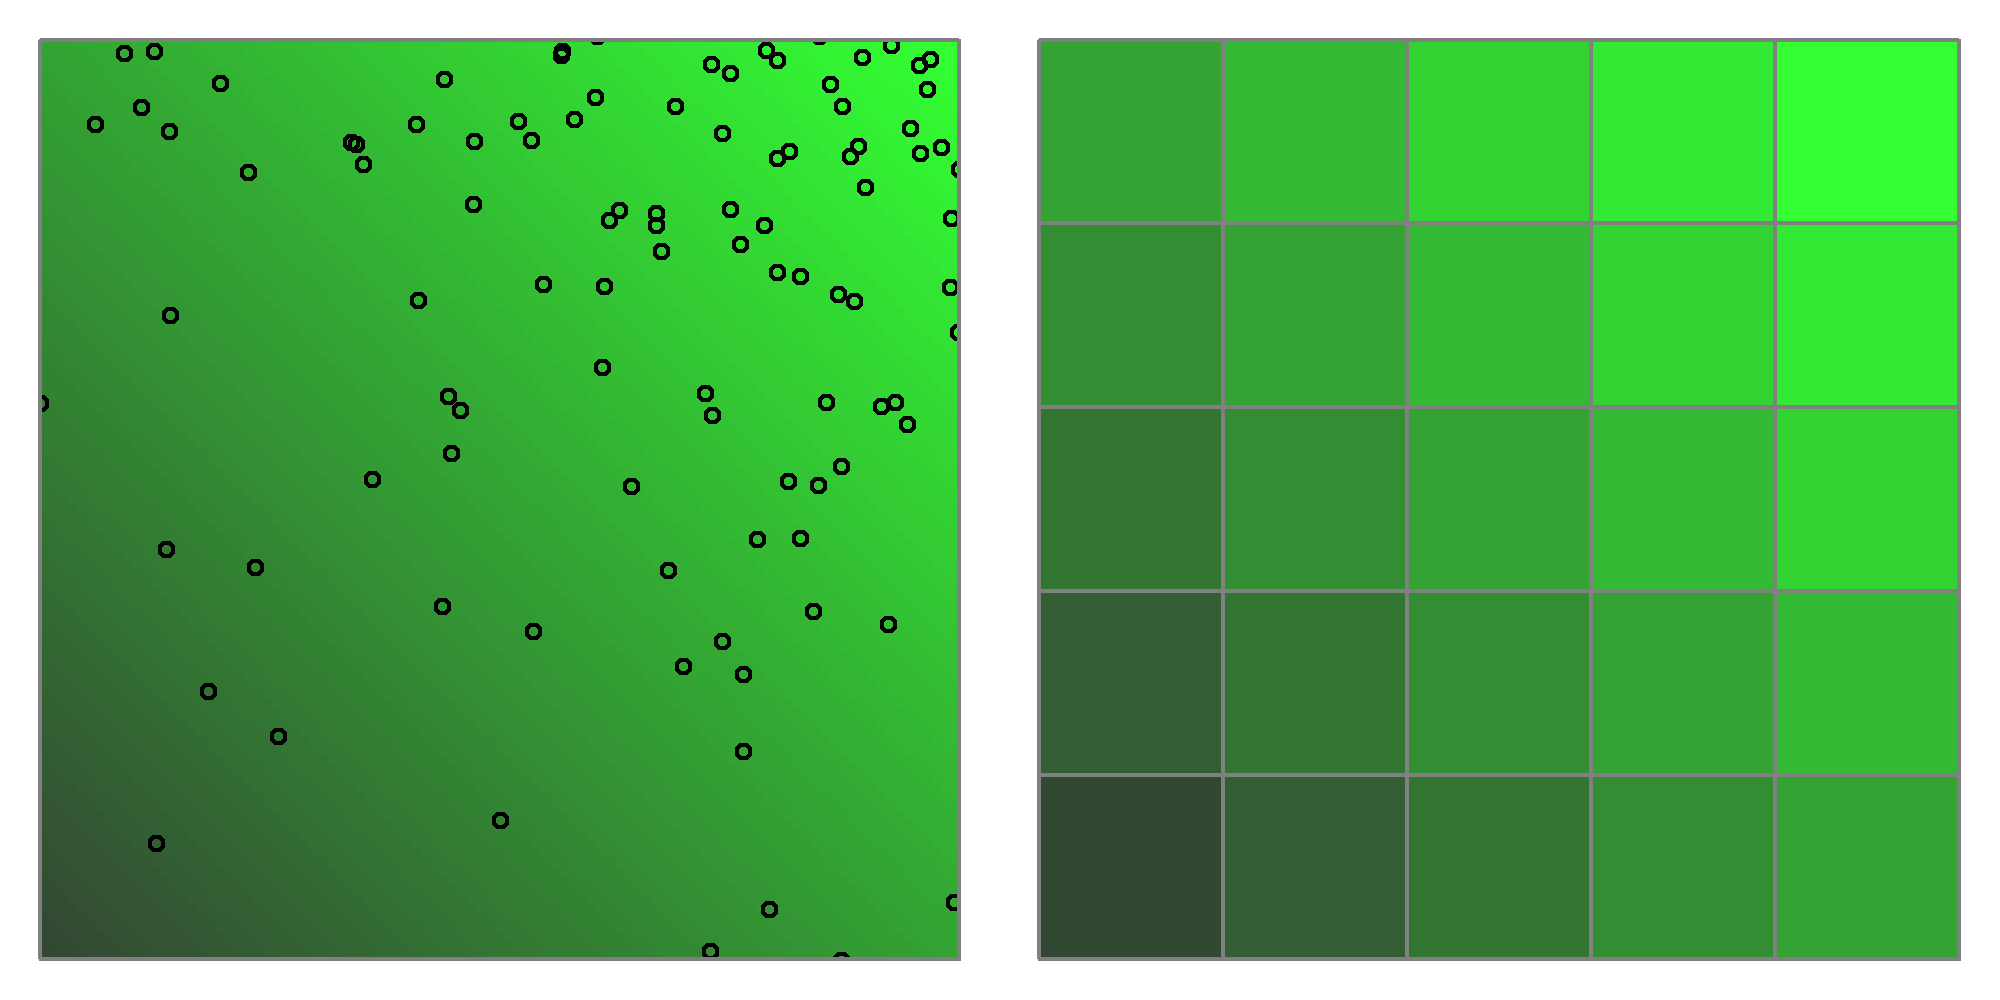
\includegraphics[width=5in,height=2.5in]{Ch11/figs/heteroPlots}
\label{state-space.fig.hetero}
\caption{An example of a spatial covariate, say elevation, and a
  realization of a inhomogeneous binomial point process with $N$=100
  and $\mu(s) = exp(\beta \mbox{elev}(s))$ where $\beta=2$.}
\end{figure}

The simulated data are shown in Fig~\ref{state-space.fig.hetero}. High elevations
are represented by light green and low elevations by dark green. The
activity centers of 100 animals are shown as
points, and it is clear that these simulated animals prefer the high
elevations.  %Perhaps they are mountain goats.
The underlying model describing this preference is
$\log(\mu(s)) = \exp(\beta \times elev(s))$
where $\beta=2$ is the parameter to be estimated.

Given these points, we will now estimate $\beta$ by minimizing the
negative-log-likelihood using \verb+R+'s \verb+optim+ function.

\begin{small}
\begin{verbatim}
# Negative log-likelihood
nll <- function(beta) {
    int.mu <- R2Cuba:::cuhre(2, 1, mu, beta=beta)$value
    -sum(beta*elev.fn(s) - log(int.mu))
}
starting.value <- 0
fm <- optim(starting.value, nll, method="Brent",
            lower=-5, upper=5, hessian=TRUE)
c(Est=fm$par, SE=sqrt(1/fm$hessian)) # estimates and SEs
\end{verbatim}
\end{small}


Maximizing the likelihood took a small fraction of a second, and we
obtained an estimate of $\hat{\beta}=1.99$. We could plug
this estimate into our linear model at each point in the state-space to
obtain the MLE for the intensity surface.

This example demonstrates
that if we had the data we wish we had, {\it i.e.} if we knew the
coordinates of the activity centers $\bf s$, we could easily estimate the
parameters governing the underlying point process. Unfortunately, in
SCR models, the activity centers cannot be directly observed, but
spatial re-captures provide us with the information needed to
estimate these latent parameters.

\section{Fitting inhomogeneous point process SCR models}

\subsection{Continuous space}

One of the nice things about hierarchical models is that they allow us
to break a problem up into a series of simple conditional
sub-models. Thus,
we can simply add the methods described above into our existing MCMC
algorithm to simulate the posterior distributions of $\beta$ conditional on the
simulated values of $\mathbf{s}$. To demonstrate, we will continue with
the previous example. Specifically, we will overlay a grid of
traps on the map shown in Fig.~\ref{state-space.fig.hetero}. We will then
simulate capture histories conditional upon the activity
centers. Then, we will attempt to estimate the activity center
locations as though we did not know where they were, as is the case in
real applications.

The following \R~code simulates encounter histories under a
Poisson observation model (see Chapt. \ref{chapt.poisson-mn}), which could be appropriate in camera
trapping studies or when using other methods in which animals could
be detected multiple times at a trap during a single occasion.

\begin{small}
\begin{verbatim}
# Create trap locations
xsp <- seq(-0.8, 0.8, by=0.2)
len <- length(xsp)
X <- cbind(rep(xsp, each=len), rep(xsp, times=len))

# Simulate capture histories, and augment the data
ntraps <- nrow(X)
T <- 5
y <- array(NA, c(N, ntraps, T))

nz <- 50 # augmentation
M <- nz+nrow(y)
yz <- array(0, c(M, ntraps, T))

sigma <- 0.1  # half-normal scale parameter
lam0 <- 0.5   # basal encounter rate
lam <- matrix(NA, N, ntraps)

set.seed(5588)
for(i in 1:N) {
    for(j in 1:ntraps) {
        distSq <- (s[i,1]-X[j,1])^2 + (s[i,2] - X[j,2])^2
        lam[i,j] <- exp(-distSq/(2*sigma^2)) * lam0
        y[i,j,] <- rpois(T, lam[i,j])
    }
}
yz[1:nrow(y),,] <- y # Fill
\end{verbatim}
\end{small}

Now that we have a simulated capture-recapture dataset $y$, and we have
augmented it to create the new data object $yz$, we are ready to
begin sampling from the posteriors. A commented Gibbs sampler written
in \R~is available in the accompanying \R~package \scrbook~(see
?scrIPP).
\begin{comment} see Ch 7 MCMC for SCR and cite some section of that \end{comment}
% There are two small parts of the
% \R~code that distinguish it from previous code we have shown to
% fit homogeneous point processes. First, we need to update the parameter
% ${\bf \beta}$ conditional on all other parameters in the model. The code to
% do so is: %\begin{comment} need cite to Ch 2 or 7 on MCMC for this \end{comment}
% \begin{small}
% \begin{verbatim}
% # Denominator of f(x, beta). Integral of mu(x, beta) over space
% D1 <- cuhre(2, 1, mu, lower=c(xlims[1], ylims[1]),
%             upper=c(xlims[2], ylims[2]), beta=beta1)$value
% # Compute the denominator again using a proposed beta1
% beta1.cand <- rnorm(1, beta1, tune[3])
% D1.cand <- cuhre(2, 1, mu, lower=c(xlims[1], ylims[1]),
%                  upper=c(xlims[2], ylims[2]), beta=beta1.cand)$value
% # Compute log(f(x))
% ll.beta1 <- sum(  beta1*elev.fn.v(S) - log(D1) )
% ll.beta1.cand <- sum( beta1.cand*elev.fn.v(S) - log(D1.cand) )
% if(runif(1) < exp(ll.beta1.cand - ll.beta1) )  {
%      beta1<-beta1.cand
% }
% \end{verbatim}
% \end{small}
% Next, we need to put the new prior on the activity centers:
% \begin{small}
% \begin{verbatim}
% # Compute the prior for s_i and a candidate. denominator is constant
% prior.S <- beta1*elev(S[i,1], S[i,2]) # - log(D1)
% prior.S.cand <- beta1*elev(Scand[1] + Scand[2]) # - log(D1)
% if(runif(1)< exp((ll.S.cand+prior.S.cand) - (ll.S+prior.S))) {
%     S[i,] <- Scand
%     lam <- lam.cand
%     D[i,] <- dtmp
%     }
% \end{verbatim}
% \end{small}
We can apply this modified sampler to our data using the
following \R~commands:
\begin{small}
\begin{verbatim}
set.seed(3434)
fm1 <- scrIPP(yz, X, M, 6000, xlims=c(0,1), ylims=c(0,1),
            tune=c(0.003, 0.08, 0.3, 0.07) )
plot(mcmc(fm1$out))
rejectionRate(mcmc(fm1$out))
\end{verbatim}
\end{small}
We obtain posterior distributions that are summarized in
Table~\ref{ch9.tab.simIPP}.
%Mixing is good, and as usual,
%life is very nice when we are working with simulated data.

\begin{table}[b]
\centering
\caption{Posterior summaries from inhomogeneous point process model
  fitted to simulated data. Space was treated as continuous.}
\begin{tabular}{lrrrrr}
\hline
& Mean & SD & 2.5\% & 50\% & 97.5\% \\
\hline
 $\sigma =0.10$ &   0.1026 &   0.0048 &   0.0935 &   0.1025 &   0.1123 \\
 $\lambda_0=0.50$ &   0.4419 &   0.0493 &   0.3496 &   0.4400 &   0.5390 \\
 $\psi =0.66$ &   0.6826 &   0.0554 &   0.5762 &   0.6820 &   0.7923 \\
 $\beta =2.00$ &   2.1601 &   0.3390 &   1.5193 &   2.1583 &   2.8043 \\
 $N =100$ & 102.7696 &   6.2689 &  92.0000 & 102.0000 & 117.0000 \\
\hline
\end{tabular}
\label{ch9.tab.simIPP}
\end{table}


Fitting continuous space IPP models is somewhat
difficult in \bugs~because our prior ``IPP'' is not one of the
available distributions that come with the software. It is
possible to add new distributions in \bugs, but it is somewhat
cumbersome.  \secr~allows
users to fit continuous space IPPs using polynomials of the x- and y-
coordinates, but it does not accept truly continuous covariates that
are functions of space. However, these
are not really important limitations because discrete
space versions of the IPP model are straight-forward, and virtually all spatial
covariates are, or can be, defined as such.


\subsection{Discrete space}
\label{modeling.sec.discrete}

To fit IPPs using covariates in discrete space, \emph{i.e.} in raster
format, we follow the same steps
as outlined in Chapter~\ref{chapt.poisson-mn}---we define ${\bf s}_i$ as
pixel ID, and we use the categorical distribution as a prior. A good
example is found in \citep{mollet_etal:2012}. Here we present
an analysis of the simulated data shown in the %right panel of
Fig.~\ref{state-space.fig.hetero}. The spatial covariate, let's call it
elevation again, was simulated
using using the code shown on the help page
\verb+ch9simData+ in \scrbook. The points are the number of
activity centers in each pixel, generated from a single realization of
the inhomogeneous point process model with intensity
$\mu(x) = 2 \times \mbox{elev}(s)$.
\begin{figure}[ht]
\centering
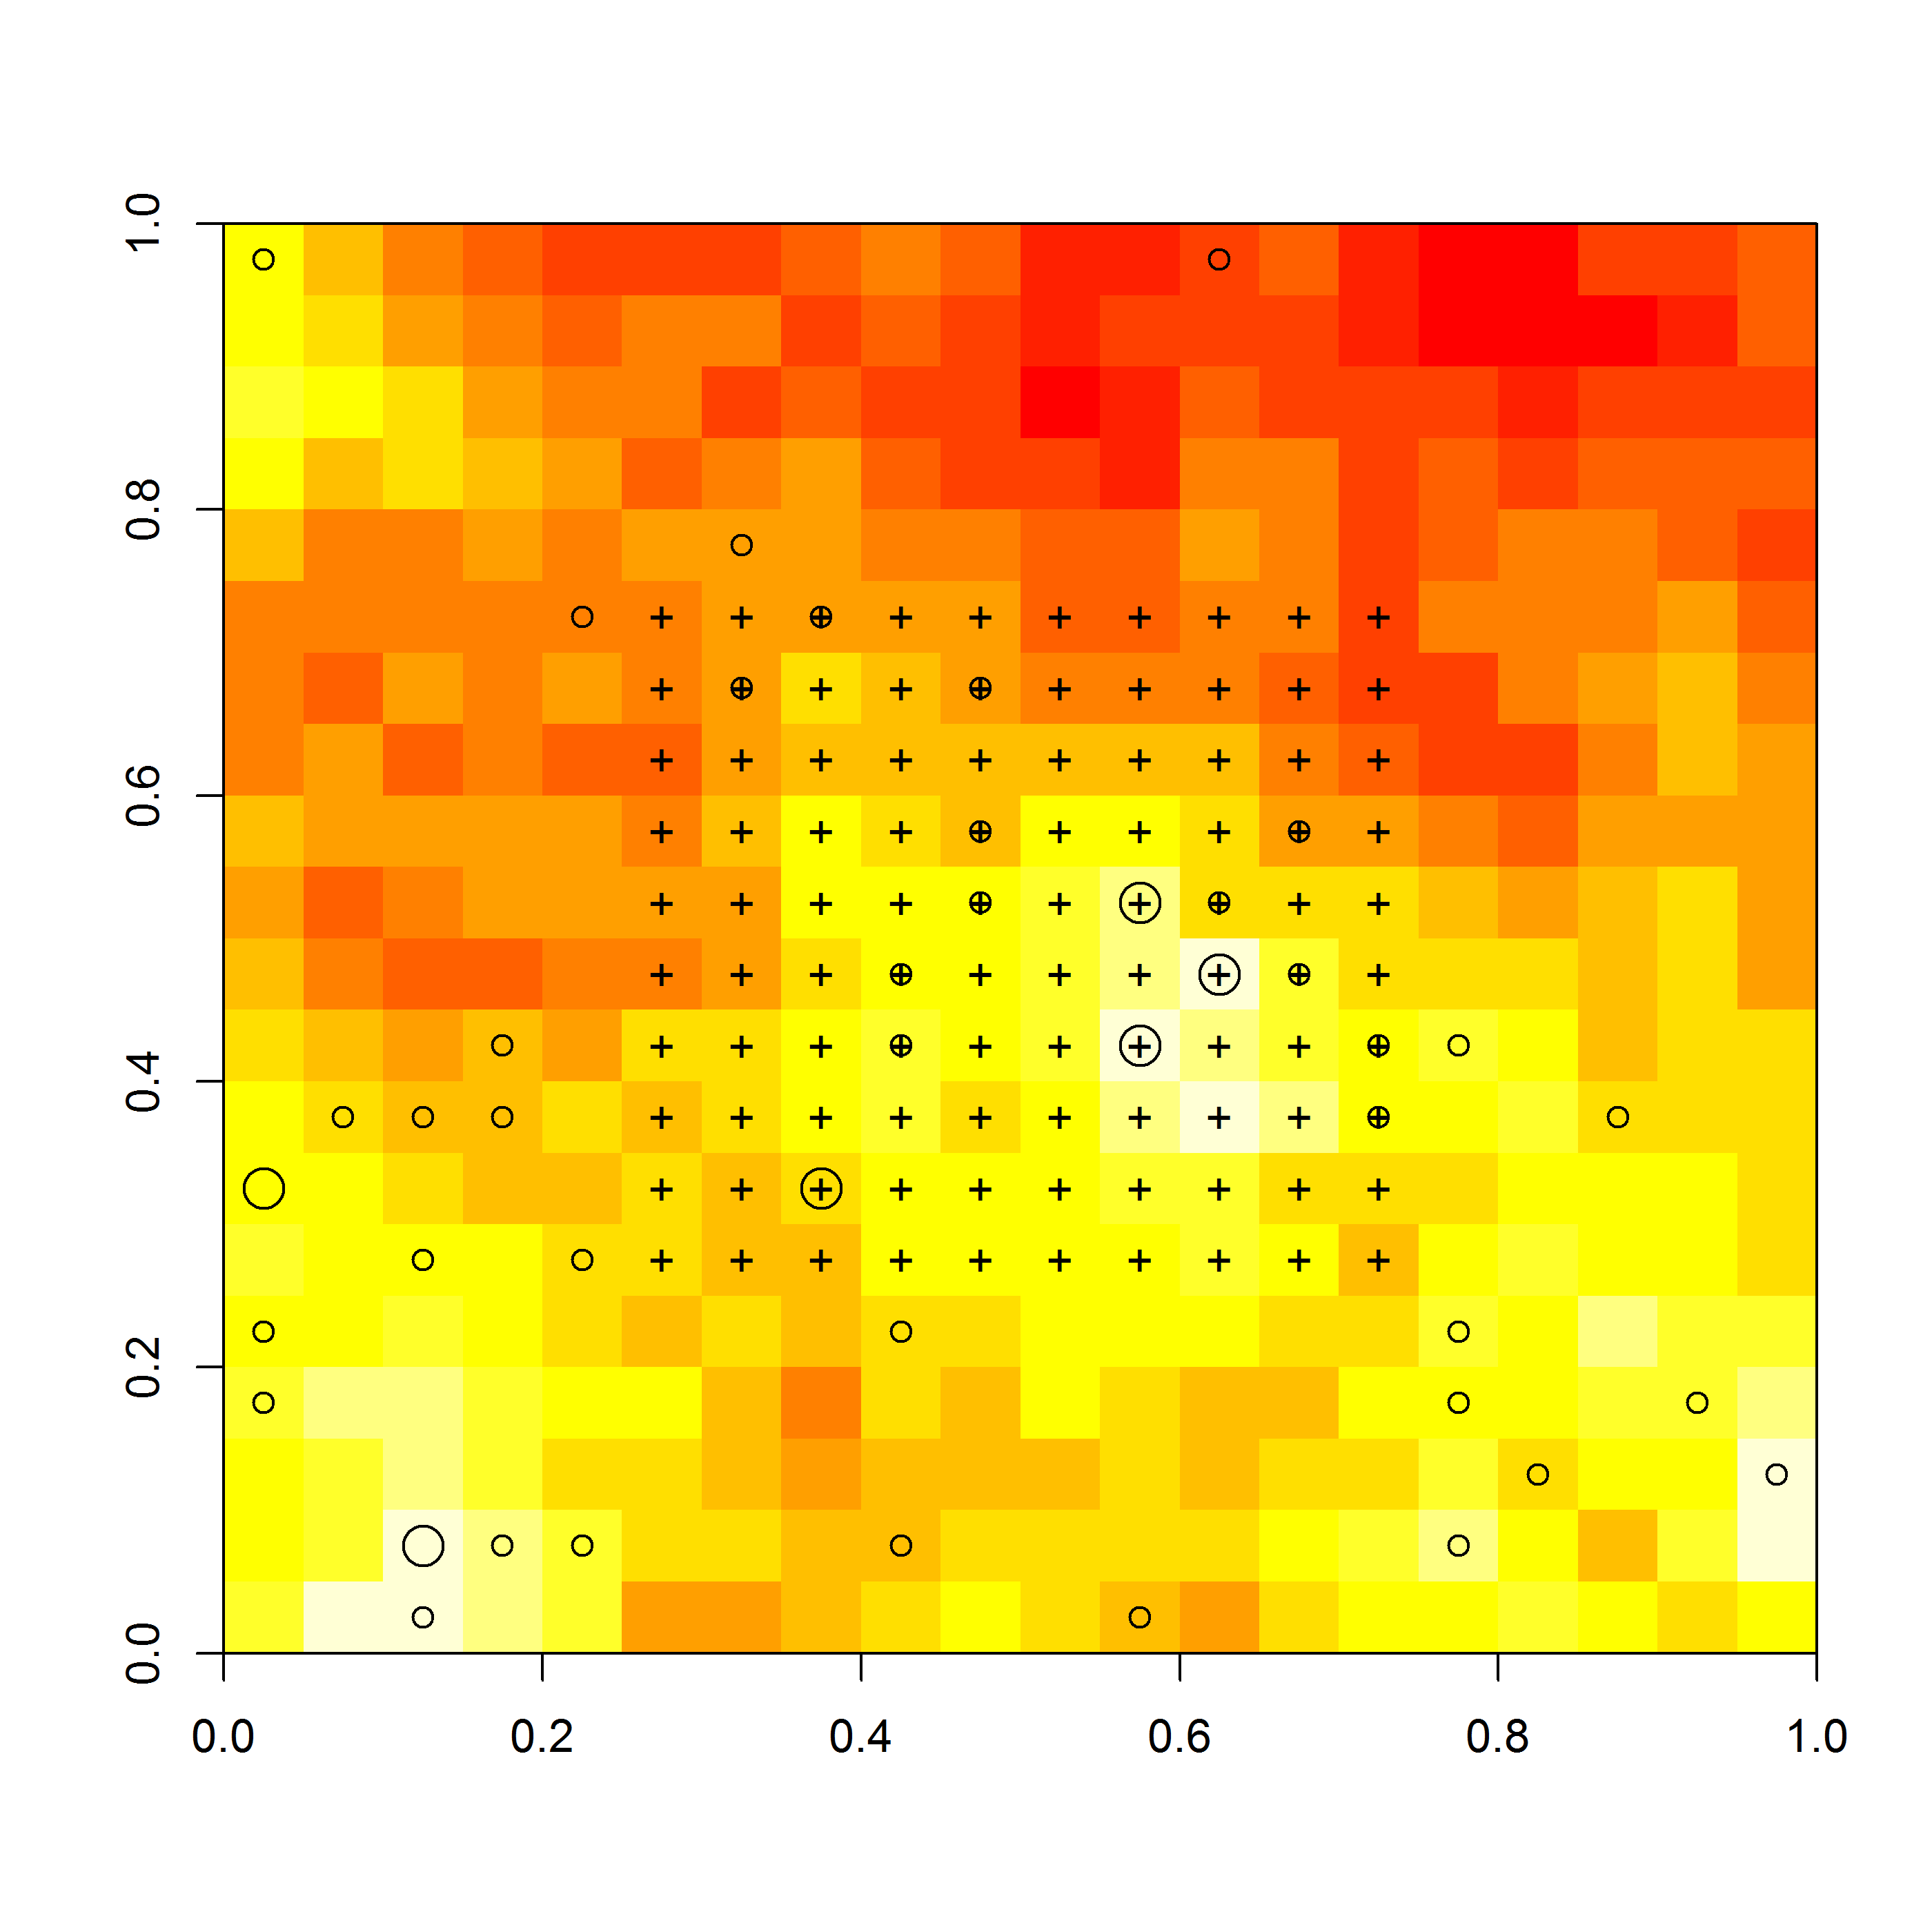
\includegraphics[width=3in,height=3in]{Ch11/figs/discrete}
\label{ch9.fig.discrete}
\caption{Simulated activity centers in discrete space. The spatial
  covariate, elevation, is highest in the lighter areas. Density of
  activity centers (circles) increases with elevation. A single
  activity center is shown as a small circle, and larger circles
  represent two activity centers in a pixel. Trap locations
  are shown as crosses.}
\end{figure}

The \bugs~code to fit an IPP model to these data is shown in
panel~\ref{ch9.panel1}.The vector \verb+probs[]+ is the prior
probability defined
by~\ref{eq.pdf.ipp.d}, which is the probability that an individual's
activity center is located at pixel $x$. \verb+Sgrid+ is the
matrix of coordinates for each pixel.

%\begin{panel}[h!]
%\centering
%\rule[0.15in]{\textwidth}{.03in}
\begin{small}
\begin{verbatim}
model{
sigma ~ dunif(0, 1)
lam0 ~ dunif(0, 5)
beta ~ dnorm(0,0.1)
psi ~ dbeta(1,1)
for(x in 1:nPix) {
  theta[x] <- exp(beta*elevation[j])
  probs[x] <- theta[j]/sum(theta[])
}
for(i in 1:M) {
  w[i] ~ dbern(psi)
  s[i] ~ dcat(probs[])
  x0g[i] <- Sgrid[s[i],1]
  y0g[i] <- Sgrid[s[i],2]
  for(j in 1:ntraps) {
    dist[i,j] <- sqrt(pow(x0g[i]-grid[j,1],2) +
                      pow(y0g[i]-grid[j,2],2))
    lambda[i,j] <- lam0*exp(-dist[i,j]*dist[i,j] /
                            (2*sigma*sigma)) * w[i]
    y[i,j] ~ dpois(lambda[i,j])
    }
  }
N <- sum(w[])
Density <- N/1 # unit square
}
\end{verbatim}
\end{small}
%\rule[0.15in]{\textwidth}{.03in}
%\caption{\bugs~code for fitting inhomogeneous point process model in
%  discrete space.}
%\label{ch9.panel1}
%\end{panel}

This model can also be fit in \secr, which refers
to the raster data as a ``habitat mask''. \R~code to
fit the models using \secr~and \jags~is available in \scrbook---see
\verb#help(ch9secrYjags)#. Results of the
comparison are shown in Table \ref{ch9:tab:secrYjags} and are
very similar as expected.
\begin{comment}
\hl{ANDY, is there any point in discussing
  the slight differences?}
  YES: If we can explain it. Could it be MC error alone?
Otherwise I guess attributing it to differences between MLE and BAyes is ok. That seems like
a reasonable thing.
\end{comment}
\begin{table}[h!]
\centering
\caption{Comparison of \secr~and \jags~results. Point estimates from
  the Bayesian analysis are posterior means. Intervals are lower and
  upper 95\% CIs.}
\begin{tabular}{llrrrr}
\hline
Software & Parameter & Estimate & SD & lower & upper \\
\hline
 secr & $N=50$ & 49.2803 & 5.7535 & 41.0087 & 64.3879 \\
      & $\beta=2$ &  2.1772 & 0.5628 &  1.0741 &  3.2804 \\
      & $\lambda_0=0.8$ &  0.9203 & 0.0764 &  0.7824 &  1.0825 \\
      & $\sigma=0.1$ &  0.0990 & 0.0038 &  0.0918 &  0.1068 \\
\hline
 JAGS & $N=50$ & 48.2072 & 5.4053 & 39.0000 & 60.0000 \\
      & $\beta=2$ &  2.1026 & 0.5323 &  1.0889 &  3.1506 \\
      & $\lambda_0=0.8$ &  0.9328 & 0.0766 &  0.7898 &  1.0921 \\
      & $\sigma=0.1$ &  0.1004 & 0.0041 &  0.0929 &  0.1089 \\
\hline
\end{tabular}
\label{ch9:tab:secrYjags}
\end{table}


\section{Ecological distance and state-space covariates}

Habitat characteristics that affect population
density could also affect home range size and movement behavior. For
example, a
species that occurs in high density in a forest may be reluctant to
venture from a forest patch into an adjacent field. Thus, even if a
trap placed in a field is located very close to an animal's activity
center, the probability of capture may be very low. In this case
forest cover is a covariate of both density and encounter probability,
and we could model it as such by combining the methods described in
this chapter and in Chapter~\ref{chapt.ecoldist}. To demonstrate, we
continue with our analysis of the data shown in
Fig~\ref{state-space.fig.hetero}. Once again, we suppose that density
increases with elevation, but this time, we also make the
assumption that home range size decreases as density increases. This
commonly-observed phenomenon can be explained by numerous factors such
as intra-specific competition \citep{sillett_etal:2004} or optimal
foraging behavior \citep{tufto_etal:1996,said_servanty:2005}. To model
this effect, we
introduce the parameter $\theta$, which determines the ``cost'' of
moving between pixels. If $\theta=0$, then the animal perceives
distance as Euclidean. If $\theta>0$, then least-cost distance (LCD)
is greater than than Euclidean distance (ED). In most cases, we would
not expect,
or should not even consider the possibility of $\theta<0$ because this
implies that LCD$<$ED, which would mean that an animal could view
1000km as 1m. In addition to the fact that this is not biologically
justifiable, it also suggests that the area of the state-space could
be infinitely large. Thus, one may want to enforce the constraint that
$\theta$ is strictly $\geq 0$. See Chapter~\ref{chapt.ecoldist} for
more details.

One may wonder if it is possible to estimate both $\beta$
and $\theta$ using standard SCR data. Currently, it is not possible to
model least-cost distance using \jags~or \secr, so we wrote our own
function, \verb+scrDED+, to fit the model using maximum likelihood. An
example analysis is provided on the help page for the function in our
\R~package \scrbook. We briefly note here that the function requires
the capture history data, the trap locations, and the raster data
formatted using the {\tt raster} package
\citep{hijmans_vanetten:2012}. The linear model for the
intensity parameter $\mu(s, \beta)$ and the least-cost distance
function $lcd(\theta)$ are specified using \R's formula interface. A
simple function call is
\begin{verbatim}
fm <- scrDED(y, traplocs=X, den.formula=~elev, dist.formula=~elev,
             rasters=elev.raster)
\end{verbatim}
To assess the possibility of estimating both $\beta$ and $\theta$, we
conducted a small simulation study, generating 500 datasets from the
model with both parameters set to 1, which corresponds to the
conditions described above. Rather incredibly, we see that it is
possible to estimate both parameters with high accuracy
(Fig~\ref{ch9.fig.sim}).

\begin{figure}[ht]
\centering
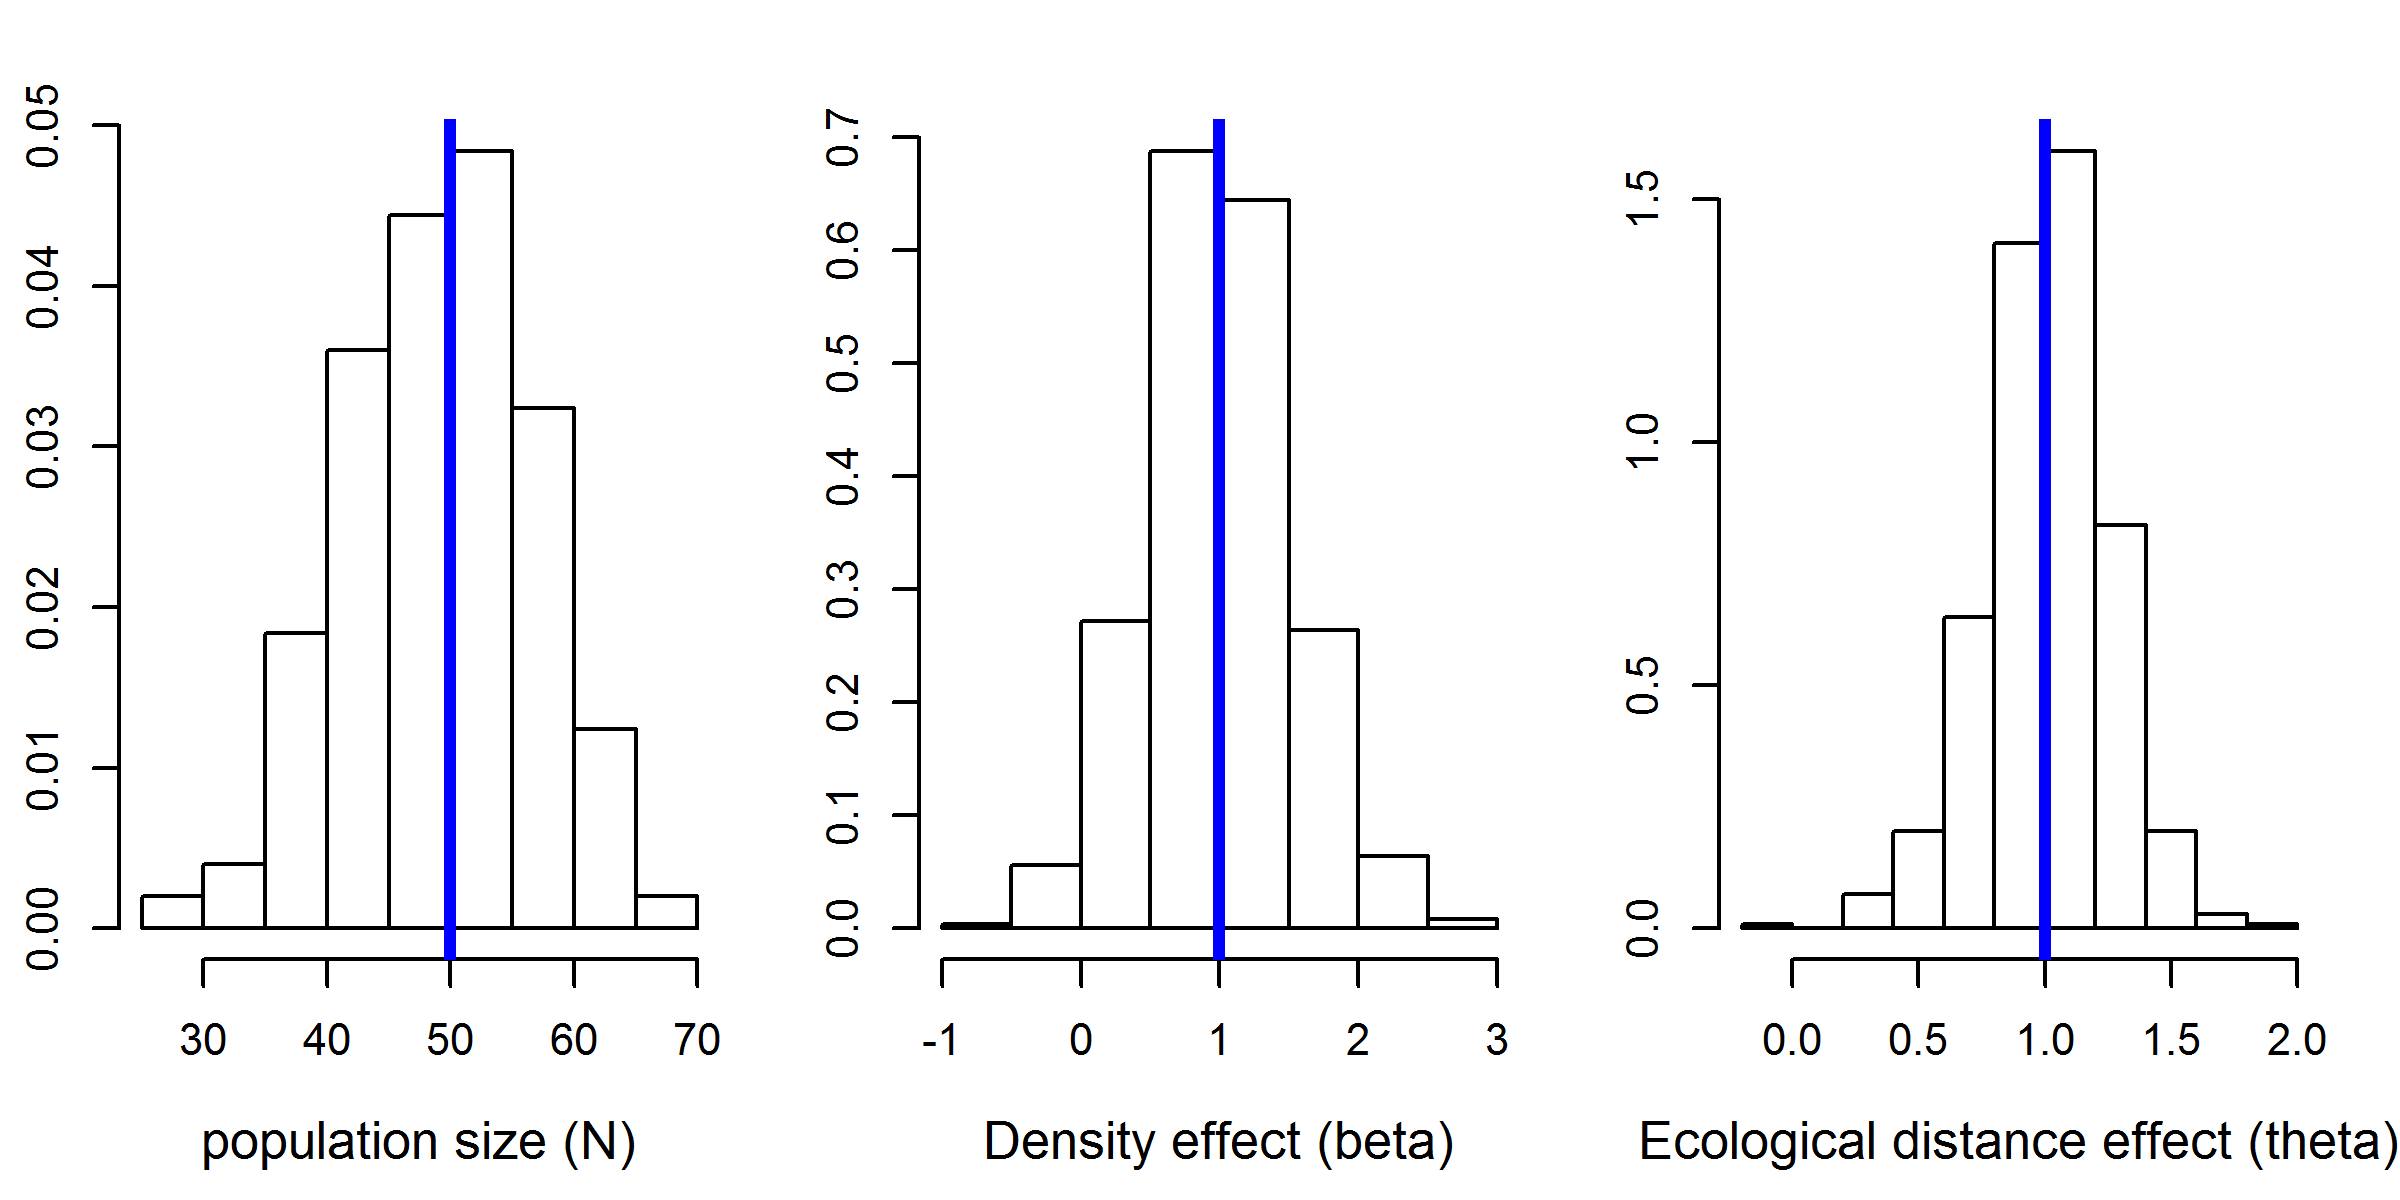
\includegraphics[width=4in,height=2in]{Ch11/figs/scrDEDsim}
\caption{Histograms of parameter estimates from 500 simulations under
  the model in which both density and ecological distance are affected
by the same covariate, elevation. The vertical lines indicate the
data-generating value.}
\label{ch9.fig.sim}
\end{figure}



\section{The jaguar data}

Estimating density of large felines has been a priority for many
conservation organizations, but no robust methodologies existed before
the advent of SCR. Distance sampling is not feasible for such rare and
cryptic species, and traditional capture-recapture methods yield
estimates that are highly sensitive to the subjective choice of the
effective survey area. In this example, we
demonstrate how readily density can be estimated for a
globally imperiled species using SCR. Furthermore, we show how
inhomogeneous point process models can be used to test important
hypotheses regarding the ecological factors affecting density.

In this example, we make use of a single year of data from an 8-year
camera-trapping study of jaguars in Argentina,
along the borders with Brazil and Paraguay. The data come from 46
camera stations, each consisting of a pair of cameras placed along
roads or trails. Forty-five detections of 16 jaguars (8 males and 8
females) were made over a 95-day sampling period. The mean number of
sampling days at each camera station was 48.2.

Estimating density is a central objective of this study because
ultimately, an estimate of the total population size for the entire
study area is needed, which can only be obtained by extrapolation of
density estimates. A second, and related, objective was to assess
the influence of poaching on jaguar density. Although jaguars
themselves are occasionally killed by poachers, the larger concern is
the influence of poaching on prey species. To protect jaguars and
related species, protected areas have
been established and three levels of protection are
recognized in the study region as depicted in Fig.~\ref{ch9.fig.jaguarCts}.

\begin{figure}[ht]
\centering
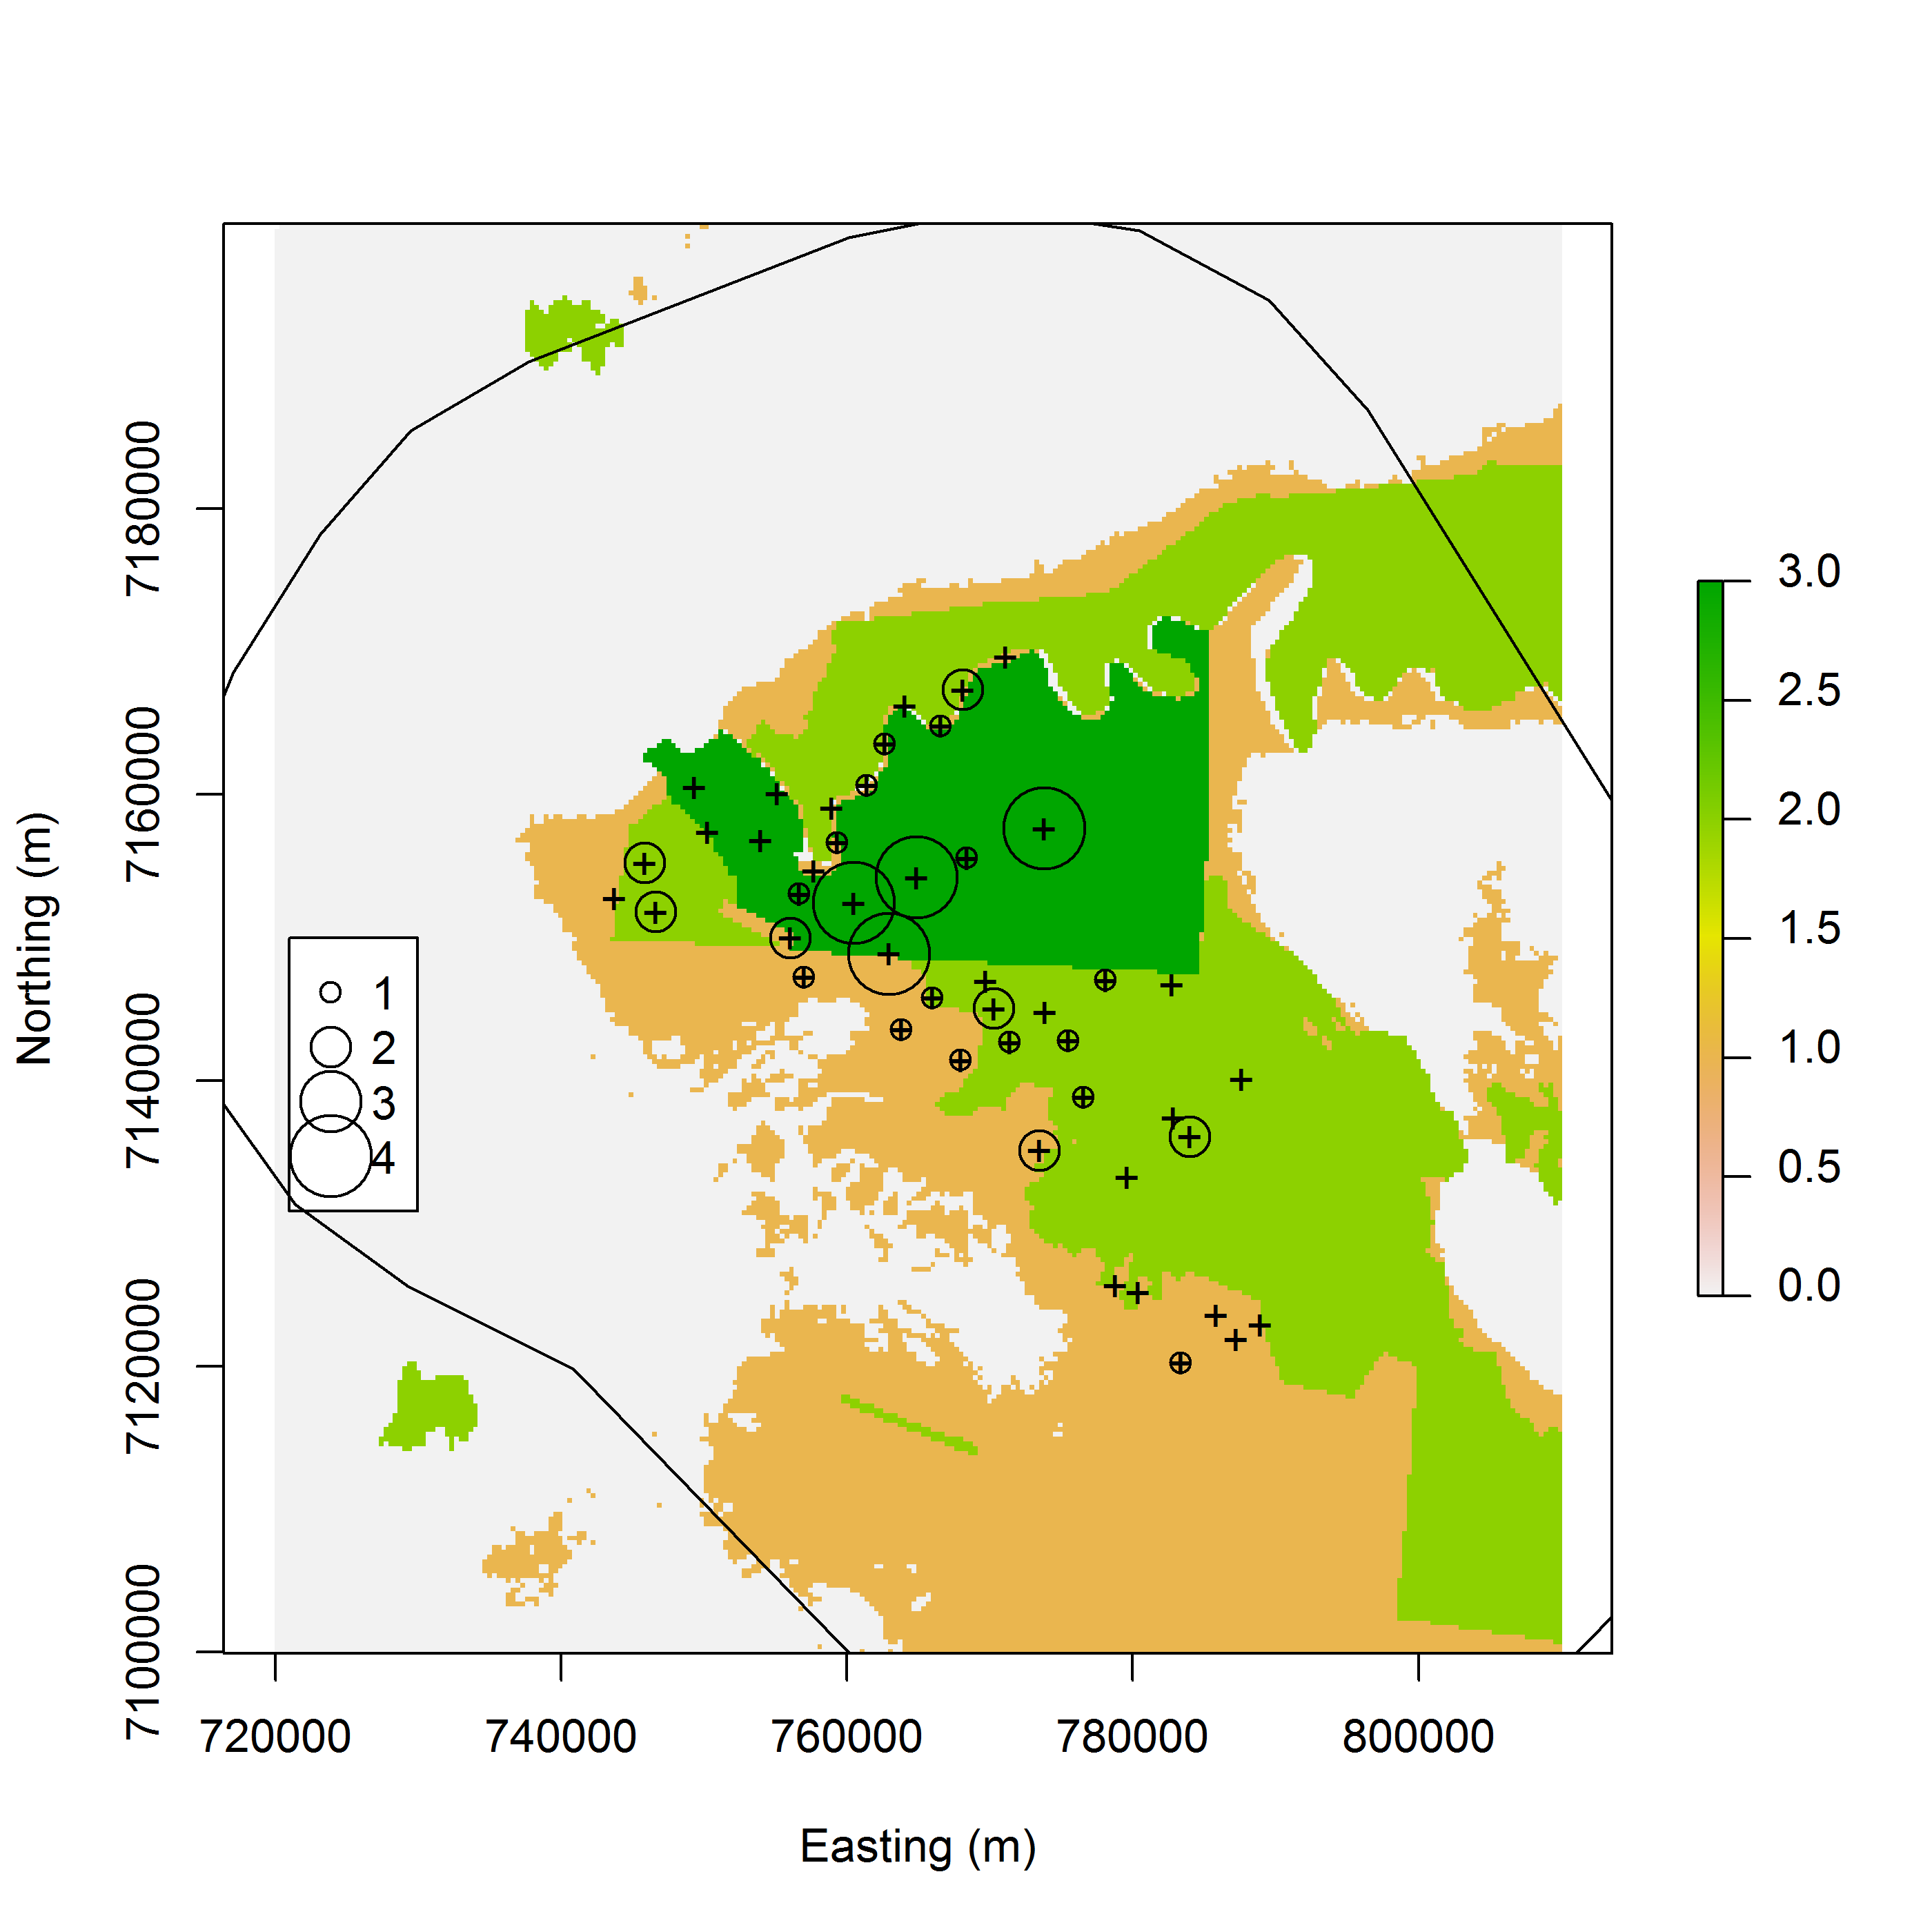
\includegraphics[width=3in,height=3in]{Ch11/figs/jaguarCountMap}
\label{ch9.fig.jaguarCts}
\caption{Jaguar detections at 46 camera trap stations. The three levels of
  protection status are no protection (beige), some protection (light
  green), and national park (dark green). Non-habitat is shown in gray
  and represents large soybean monocultures. }
\end{figure}

To assess the influence of poaching on jaguar density, we treated
protection status as an ordinal variable with 3 levels: no protection,
some protection, and high protection (national parks). Clearly these
are ordered, and our
hypothesis is that poaching pressure should decrease and jaguar
density should increase with the level of
protection. Thus, $\beta$ in this example is a ``slope''
parameter describing the degree to which protection status affects
jaguar density. We also hypothesized that males and females could have
different home range sizes and that the sex ratio may not be
1:1. Furthermore, we restricted the state-space to exclude the large
soybean monocultures surrounding the study area, and we only
considered
area south of the Iguazu River, which runs along the northern border
of the park shown in dark green in
Fig.~\ref{ch9.fig.jaguarCts}. Rather than restricting the
state-space, we could have modeled the permeability of the river using
the methods described in the previous section and in
Chapter~\ref{chapt.ecoldist}; however, no sampling was conducted on
the northern side of the river, and ancillary data indicates that
jaguars very rarely forge the waterway. \R~code to fit the model is
available in \scrbook  on the help page \verb+jaguarDataCh9+. Parameter
estimates are shown in Table\ref{ch9.tab.jagposts}.
\begin{table}
\centering
\caption{Summaries of posterior distributions from the model of jaguar
  density. $\sigma_f$ and $\sigma_m$ are the scale parameters of
  the half-normal detection function for females and males
  respectively. $\rho$ is the
  sex-ratio. $\lambda_0$ is base-line encounter rate. $\beta$ is the
  effect of protection on jaguar density. D is the overall density
  estimate. D1, D2, and D3 are the density estimates
  (jaguars/100km$^2$) for the three levels of protection. }
\begin{tabular}{lrrrrr}
\hline
& Mean & SD & 2.5\% & 50\% & 97.5\% \\
\hline
 $\sigma_f$ &  7361.731 &  1907.566 &  4899.740 &  7002.770 & 12083.110 \\
 $\sigma_m$ &  8177.068 &  1545.717 &  5916.151 &  7955.788 & 11842.486 \\
 $\rho$ &     0.516 &     0.118 &     0.286 &     0.516 &     0.741 \\
 $\lambda_0$ &     0.007 &     0.002 &     0.003 &     0.007 &     0.012 \\
 $\beta$ &     4.405 &     1.443 &     2.553 &     4.143 &     7.775 \\
 D &     0.533 &     0.708 &     0.000 &     0.000 &     0.072 \\
 D1 &     0.132 &     0.010 &     0.095 &     0.095 &     0.616 \\
 D2 &     1.415 &     0.050 &     0.214 &     0.531 &     1.503 \\
 D3 &     3.516 &     0.000 &     0.292 &     3.105 &     4.220 \\
\hline
\end{tabular}
\label{ch9.tab.jagposts}
\end{table}

Our results
indicate that efforts to protect jaguars by reducing poaching are
working. Density was $>$26 times higher in the national park than in the
unprotected area. Fig.~\ref{ch9:fig:Dsurface} shows the estimated
density surface.

\begin{figure}[ht]
\centering
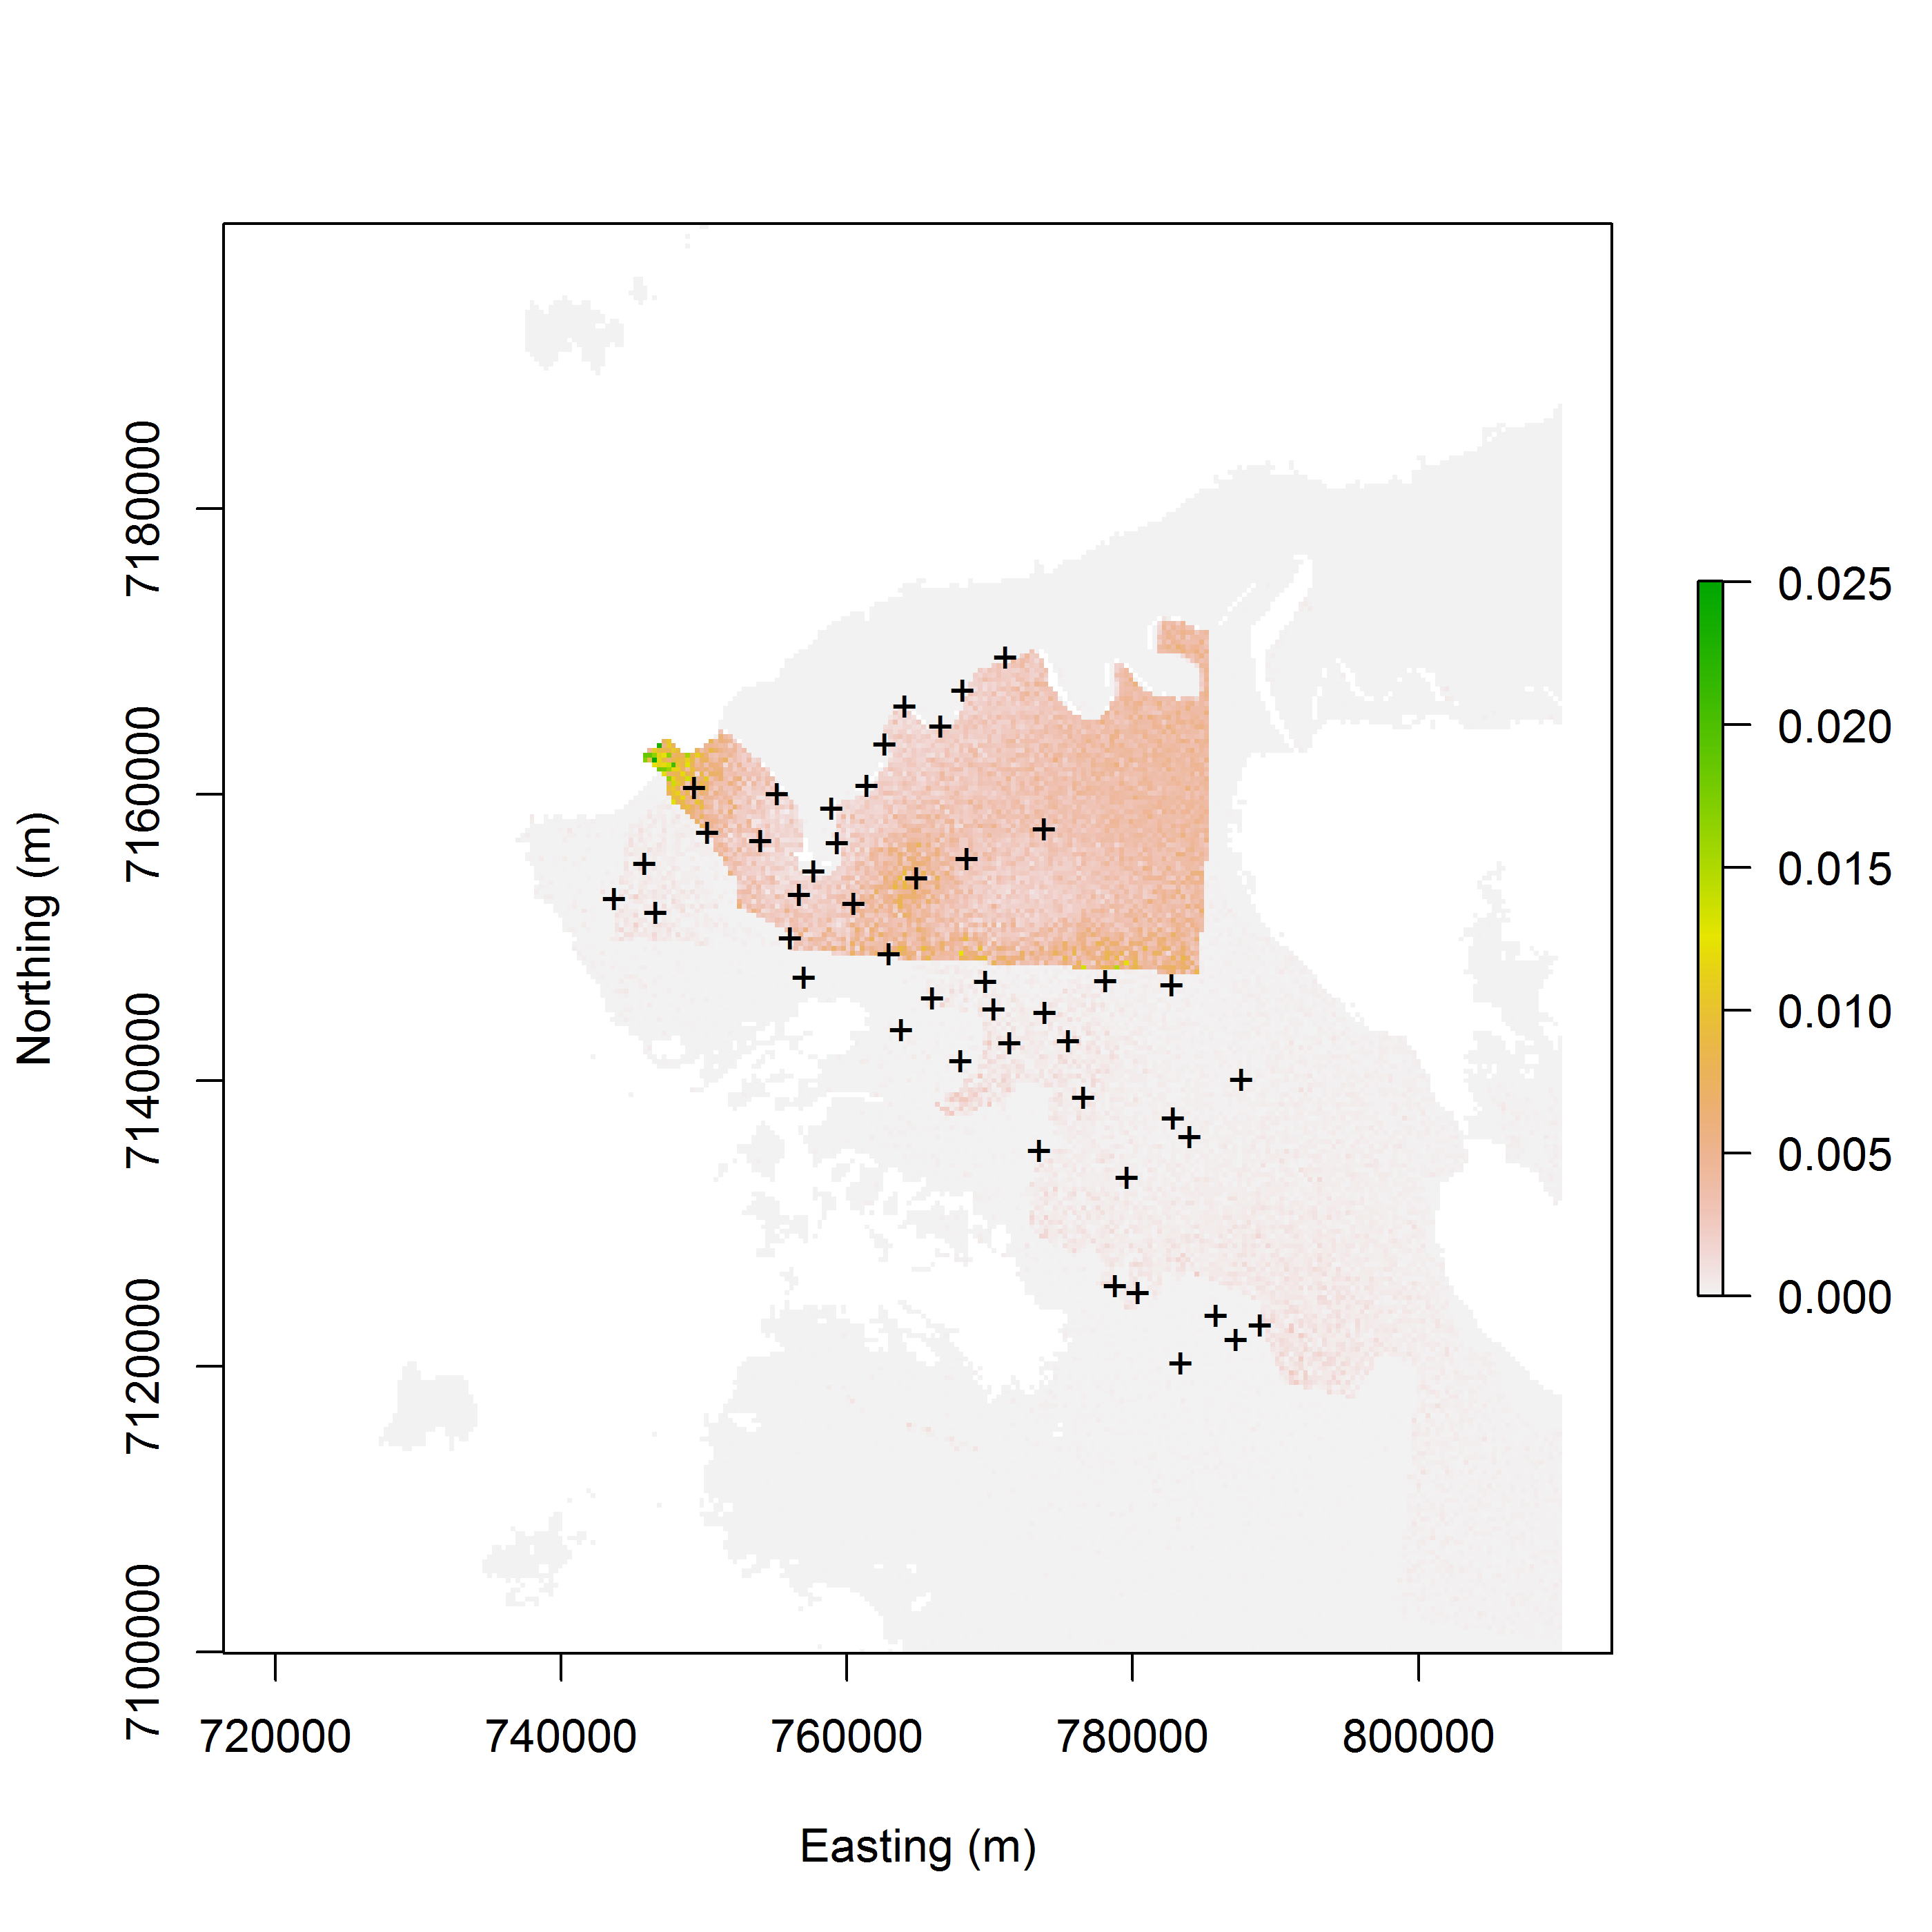
\includegraphics[width=3in,height=3in]{Ch11/figs/Dsurface34}
\label{ch9:fig:Dsurface}
\caption{Estimated density surface for the jaguar dataset}
\end{figure}


We note that there is room for improvement in our analysis. The
political boundaries used to demarcate protected areas are not as
concrete as we might like. In reality poaching pressure is likely to
be higher near remote park boundaries than in well-guarded park
interiors. One option
for addressing this would be to use a continuous measure of poaching
pressure such as distance from the nearest town, or some other
accessibility metric. It would also be interesting to model density
separately for each sex. Many of the detections outside of the park
were of males, and thus it is possible that the sexes use habitat
differently. Developing models for these two hypotheses could be
readily accomplished using slight modifications of the code found in
the \R~package \scrbook.



\section{Summary}

When state-space covariates are available,
density can be modeled by replacing the uniform prior on the activity
centers with a
prior based on a normalized log-linear function of covariates. This
distribution has been widely used in ecology to model point processes
as well as resource selection probability functions
\citep{manly_etal:2002,lele_keim:2006}. In the SCR
context, use of this new prior results in
a model for the inhomogeneous point process describing the
location of activity centers, which can be used to test hypotheses
about spatial variation in density. In
rare cases, these covariates are truly continuous in the sense that
they are defined as a function of space. More often, covariates are
represented as rasters, which simplifies the analysis. Fitting these
models can be accomplished using \bugs, \secr, or the custom \R~code
presented in this chapter and found in the package \scrbook.
%However,
%at the time this book was written, \scrbook is only software available
%for fitting models with covariates of both density and ecological
%distance.

All the examples in this section included a single state-space
covariate, but this was for simplicity only. Including multiple
covariates poses no additional challenges. Similarly, additional model
structure such sex-specific encounter rate parameters or behavioral
responses can be accommodated. Even more remarkable is the ability to
consider covariates that affect both density and ecological
distance. The ramifications of this are enormous for applied
ecological research and conservation efforts because, for instance,
researchers can use capture-recapture data to identify areas where
density is high, and to model important quantities such as landscape
connectivity \citep{royle_etal:2012ecol}. Addressing such questions
is simply not possible using standard, non-spatial capture-recapture
methods. Accomplishing these goals will of course require more data
than is needed to estimate the parameters of a basic SCR model.

